%%%%%%%%%%%%%%%%%%%%%%%%%%%%%%%%%%%%%%%%%
% Journal Article
% LaTeX Template
% Version 1.3 (9/9/13)
%
% This template has been downloaded from:
% http://www.LaTeXTemplates.com
%
% Original author:
% Frits Wenneker (http://www.howtotex.com)
%
% License:
% CC BY-NC-SA 3.0 (http://creativecommons.org/licenses/by-nc-sa/3.0/)
%
%%%%%%%%%%%%%%%%%%%%%%%%%%%%%%%%%%%%%%%%%

%----------------------------------------------------------------------------------------
%	PACKAGES AND OTHER DOCUMENT CONFIGURATIONS
%----------------------------------------------------------------------------------------

\documentclass[journal]{IEEEtran}



\usepackage[sc]{mathpazo} % Use the Palatino font
\usepackage[T1]{fontenc} % Use 8-bit encoding that has 256 glyphs
\usepackage[utf8]{inputenc}
\linespread{1.05} % Line spacing - Palatino needs more space between lines
\usepackage{microtype} % Slightly tweak font spacing for aesthetics
\usepackage{graphicx}
\usepackage[hmarginratio=1:1,top=32mm,columnsep=20pt]{geometry} % Document margins
\usepackage{multicol} % Used for the two-column layout of the document
\usepackage[hang, small,labelfont=bf,up,textfont=it,up]{caption} % Custom captions under/above floats in tables or figures
\usepackage{booktabs} % Horizontal rules in tables
\usepackage{float} % Required for tables and figures in the multi-column environment - they need to be placed in specific locations with the [H] (e.g. \begin{table}[H])
\usepackage{hyperref} % For hyperlinks in the PDF

\usepackage{lettrine} % The lettrine is the first enlarged letter at the beginning of the text
\usepackage{paralist} % Used for the compactitem environment which makes bullet points with less space between them

\usepackage{abstract} % Allows abstract customization
\renewcommand{\abstractnamefont}{\normalfont\bfseries} % Set the "Abstract" text to bold
\renewcommand{\abstracttextfont}{\normalfont\small\itshape} % Set the abstract itself to small italic text

\usepackage{titlesec} % Allows customization of titles
\renewcommand\thesection{\Roman{section}} % Roman numerals for the sections
\renewcommand\thesubsection{\Roman{subsection}} % Roman numerals for subsections
\titleformat{\section}[block]{\large\scshape\centering}{\thesection.}{1em}{} % Change the look of the section titles
\titleformat{\subsection}[block]{\large}{\thesubsection.}{1em}{} % Change the look of the section titles

\usepackage{fancyhdr} % Headers and footers
\pagestyle{fancy} % All pages have headers and footers
\fancyhead{} % Blank out the default header
\fancyfoot{} % Blank out the default footer
\fancyhead[C]{LINGI2141 - Individual Project $\bullet$ December 2013 } % Custom header text
\fancyfoot[RO,LE]{\thepage} % Custom footer text

%----------------------------------------------------------------------------------------
%	TITLE SECTION
%----------------------------------------------------------------------------------------

\title{\fontsize{24pt}{10pt}\selectfont\textbf{LINGI2141 - Individual Project \\Analysis of JDownloader}} % Article title

\author{
\large
\textsc{Julien Colmonts}\\[2mm] % Your name
\normalsize Université Catholique de Louvain \\ % Your institution
}
\date{}

%----------------------------------------------------------------------------------------

\usepackage{biblatex}
\bibliography{project}

\begin{document}

\maketitle % Insert title

\thispagestyle{fancy} % All pages have headers and footers

%----------------------------------------------------------------------------------------
%	ABSTRACT
%----------------------------------------------------------------------------------------

\begin{abstract}

This paper will deal with analysing the networked application JDownloader \ref{JDlr} which is a download manager for a large number of hosting sites. That kind of download manager helps people to download a large number of files from all categories. JDownloader is a cross-platform program written in the Java programming language. It supports about 110 one-click hosting sites, is able to solve some CAPTCHAs, can deal with several parallel downloads and multiple connections. It is also free and open-source.

\end{abstract}

%----------------------------------------------------------------------------------------
%	ARTICLE CONTENTS
%----------------------------------------------------------------------------------------


\section{Introduction}

\lettrine[nindent=0em,lines=3]{F}or a few years, a very large number of hosting sites has emerged. Most of them are used to exchange illegal content like movies, games, etc. Links to access this content will then be shared on different websites. With JDownloader, users aren't obliged to open these links one by one, wait the required time to be allowed to download for free and maybe fill a CAPTCHA. They can add all their links into the application and it will perform a major part of these actions by itself. As a concrete example of JDownloader use, a user just has to start the application and copy the link to the file (on the hosting site) he wants to download in his clipboard. JDownloader will automatically search if the link is valid It means that the link still exists and the file hasn't been deleted by the host (often for copyright infringement). Then, the user just has to start the download operation by clicking the play button and fill the CAPTCHA if the application can't solve it. The application is able to parse a long html code and to find all links contained in that code. The objective of analysing such an application obviously isn't to promote piracy on the internet. The idea is to understand how this download managers work. If hosts could detect they are accessed by one, they could improve their security policies. Preventing access to illegal content is a good way to fight piracy on the internet. 

%------------------------------------------------

\section{JDownloader and IPv6}
 JDownloader is still implemented to support only \textsc{IPv4} but developers are thinking to develop \textsc{IPv6} support throughout \ref{IPv6}. Project manager says that switching from one addressing method to another shouldn't be too hard because it affects only the implementation of low level layer of the application. Since it works as a web browser to reach websites, only the way of opening connections has to be modified. The main problem stands in the fact that it handles a large numbers of websites and these don't support \textsc{IPv6} yet. 

%------------------------------------------------

\section{Adding a link}
As said before, the application is able to monitor your clipboard. If a user copies an url, it will automatically check if it can download files from this address. To perform this operation, the application works as a web browser. It first needs the \textsc{IP} address of the domain written in the url so it will perform two queries to the DNS. The first one asks for \textsc{IPv4} when the second one asks for \textsc{IPv6} addresses.  \\
\begin{figure}
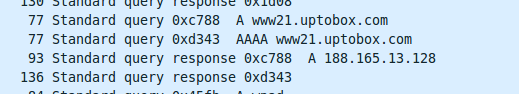
\includegraphics[scale=0.4]{dns.png}
\end{figure}

In the trace shown by Wireshark, we can see that the url \url{www21.uptobox.com} has an \textsc{IPv4} address which is $188.165.13.128$ but no \textsc{IPv6} address. 
After a three-way handshake, it will send a \textsc{GET} request in \textsc{HTTP 1.1} protocol. Since \textsc{IPv6} isn't implemented yet, it will use the first \textsc{IPv4} address which is returned by the DNS queries. Then, the page content is downloaded. In this case, the bit-rate can't be restricted. Finally, the application will send a \textsc{OK HTTP 1.1} standard message to tell the server that everything worked fine and close the connection. On the screen, the user will just see that the application is searching for a file to download. If it finds something, it displays a list of what it found. \\
If we analyse the packet that are exchange, we can observe the content of the webpage.\\
\begin{figure}[ht]

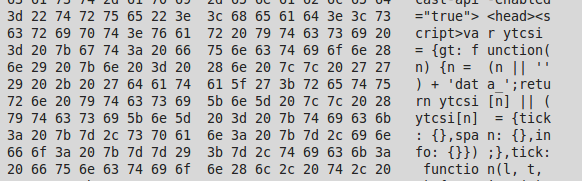
\includegraphics[scale=0.36]{htmlcode.png}
\end{figure}
In this figure, we can see the html code which is sent by the server.

%------------------------------------------------

\section{Download a link}
The main functionality of JDownloader is its ability to download files from hosting sites. When a user will add in a link as told before, the application will download the page again. During the previous operation, it only checked that files where available on the link the user gave. In this operations, the Java client has to find the address of the file to download. Parsers are implemented in the JDownloader sources to search after this address for a large number of hosts. To understand how these exchanges work, we tried to download a random dll file on a host which is called \textsc{UpToBox}. We used this host because \textsc{JDownloader} is able to avoid free accounts waiting time and to solve CAPTCHA sequences. After the page analysis, another connection is opened. \\
\begin{figure}[ht]
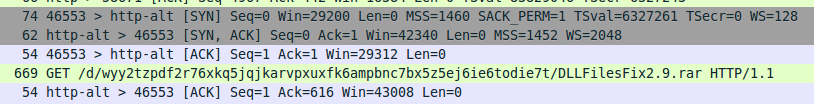
\includegraphics[scale=0.3]{dlLink.png}\\
\end{figure}
\begin{itemize}
\item The port used is an alternative to internet HTTP traffic , it's $8080$ instead of the usual $80$. 
\item The windows are significantly larger than for the first page download. The among of data which will be transmitted seems to be a relevant variable to explain this sizes. 
\item The url that is contacted contains a dynamic generated link created by the host. 
\end{itemize}
Then the download starts. 



%------------------------------------------------

\section{Update the application}

%----------------------------------------------------------------------------------------
%	REFERENCE LIST
%----------------------------------------------------------------------------------------


\printbibliography

%----------------------------------------------------------------------------------------



\end{document}
